
\section{Theory of Games}

\begin{frame}[standout]
    \onslide<+->
    \customFigure[0.42]{
        
\includegraphics{Documents/250307 BIP Portorož SI/Figures/ScrollsAndBooks_87_t.PNG}
    }{We found a book!}{We found a book!}
\end{frame}

\begin{frame}{\insertsection}
    \onslide<+->
    \begin{multicols}{2}
        The four basic elements forming a game \cite{schell2019ArtGameDesign}:
    
        \begin{itemize}
            \item mechanics -- create the structure of the game and define how players interact with it;
            \item story -- provides context and meaning to the gameplay experience;
            \item aesthetics -- contributes to the game's atmosphere and style;
            \item technology -- used to create and run the game.
        \end{itemize}

        \columnbreak

        \begin{center}
            \onslide<2->
                
\includegraphics[width=0.4\linewidth]{Documents/250307 BIP Portorož SI/Figures/mechanics.jpg}
            \hspace{1em}
            \onslide<3->
                
\includegraphics[width=0.4\linewidth]{Documents/250307 BIP Portorož SI/Figures/story.jpg}
    
            \vspace{1em}
            
            \noindent
            \onslide<4->
                
\includegraphics[width=0.4\linewidth]{Documents/250307 BIP Portorož SI/Figures/aesthetics.jpg}
            \hspace{1em}
            \onslide<5>
                
\includegraphics[width=0.4\linewidth]{Documents/250307 BIP Portorož SI/Figures/technology.jpg}
        \end{center}
        
    \end{multicols}
\end{frame}



\begin{frame}[standout]
    \onslide<+->
    \customFigure[0.42]{
        
\includegraphics{Documents/250307 BIP Portorož SI/Figures/rune_06_t.PNG}
    }{We are shown the decision-support rune.}{We are shown the decision-support rune.}
\end{frame}

\subsection{Game Theory}

\begin{frame}{\insertsection\ \insertsubsection}
    \onslide<+->

    \alert{Game Theory} studies \alert<2>{strategic interactions} between \alert<3>{rational} \alert<4>{decision-makers}.

    \vspace{2em}

    Key elements:
    \begin{multicols}{4}
        \centering
        players

        strategies

        payoffs

        equilibria
    \end{multicols}
\end{frame}

\begin{frame}[standout]
    \onslide<+->
    \customFigure[1]{
        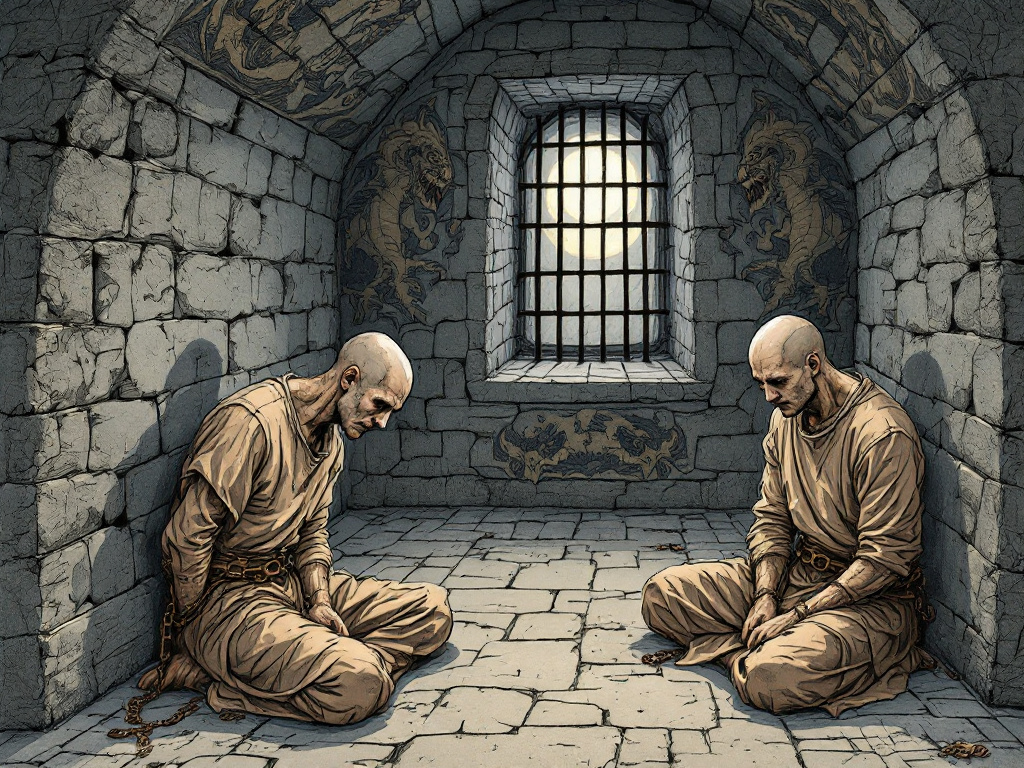
\includegraphics{Documents/250307 BIP Portorož SI/Figures/prisoners.jpg}
    }{Oh no, there's prisoners here!}{Oh no, there's prisoners here!}
\end{frame}

\begin{frame}{\insertsection\ \insertsubsection}
    \onslide<+->

    \begin{exampleblock}{Prisoner’s Dilemma}
        The classic model of cooperation vs self-interest.
    \end{exampleblock}
\end{frame}

\begin{frame}{\insertsection}
    Game Theory in Traditional Games
Zero-sum games (chess) vs. non-zero-sum (Pandemic).

Perfect information (visible moves in Go) vs. imperfect information (hidden cards in poker).

Mixed strategies: Bluffing in poker to avoid predictability.

Minimax theorem: Optimizing worst-case outcomes (used in AI for games like chess).


\end{frame}
